\section{The centralized state of the world}
\label{sec:intro}
How we communicate, how we buy and sell goods and services and even how we store our valuable information, is centrally controlled and manipulated. As George Orwell foresaw in his book \textit{1984} \cite{orwell2009nineteen}, \textit{``He who controls the past, controls the future; and he who controls the present, controls the past''}. A centralized internet creates a dangerous world with too much power in the hands of a largely unaccountable few.


\subsection{The centralized state of the internet}
\label{sec:introInternet}
The internet is centralized at every layer: from the foundational hardware stack that supports it and how all of the data within it is processed and stored, to how we access the internet, and how its power is harnessed and leveraged via browsers and applications.

\subsubsection{Centralization of access}
\label{sec:introaccess}
Access to the internet globally is granted via entrenched Internet Service Providers, with only 3 or 4 choices in each market. These providers control internet access parameters such as bandwidth, uptime, and connectivity. They do this by providing homes with broadband or similar internet services, and through 3G, 4G and 5G mobile services. There is no ability for a citizen to simply access the internet without accessing it through centralized (often state-controlled) companies. In several countries, like the Philippines, Facebook controls access through its Internet.Org initiative \cite{SoftpediaFace}. Whilst access to Facebook and its services are unrestricted, the internet outside of its own domain is severely limited. Despite its importance to every facet of modern life, the internet for many, is not a human right, but a commercial right.

Once connected, three companies control the distribution of apps - and their resulting revenue streams - on almost every one of the world's three billion smartphones and home-pods. In terms of access to content, over the past 5 years, Google and Facebook alone have crept from managing 50\% of the traffic to top web publishers, to 70\% today \cite{Newsweek2017}.

\subsubsection{Centralization of processing, storage and infrastructure}
\label{sec:introdata}
Almost two-thirds of the internet's data is stored and processed on servers owned and controlled by just four global institutions (Figure \ref{fig:internetDist}).

\begin{figure}[h]
	
\includegraphics[width=\linewidth, trim= 0cm 0cm 0cm 0cm, clip]{Figures/internetDist.png}
	\caption{The distribution of internet data storage.}
	\label{fig:internetDist}
\end{figure}
Further, despite the ever growing distribution of power production through, for example, home-based solar panels, the vast majority of worldwide power comes from centralized sources such as oil, nuclear and coal \cite{Statista2019}. As we have seen in Venezuela, in the event of a power outage, the entire internet also falls away, and with it goes the use of any blockchain, network or token.

\subsection{The dangers related to the Internet of Things (IoT)}
\label{sec:introiot}
The IoT market has exploded in the last few years, boosted by a new generation of closed and heterogeneous technologies and services, such as Z-Wave, Zigbee, LORA, Wi-Fi, Bluetooth, and Home Connect. As a result, we have seen the rise of homepod devices like Amazon's Alexa\textsuperscript{TM} or Google Home\textsuperscript{TM}, which have emerged as the dominant hubs for smart home connected hardware.

We also now live in an era where surveillance capitalism is in a symbiotic relationship with advertising technology. The current homepod offerings are cloud-based, with their \textit{modus operandi}: being to continuously record, eavesdrop on, and commoditize users' personal data. This very model is - by design - a threat to the privacy of individuals within their own homes.

As control of more and more user data continues to empower the technology giants, it also provides a global surveillance platform for the world's governments. It is naive to assume this will not eventually be compromised, or that this hasn't happened already. This accumulation of data is, in and of itself, not only a personal privacy issue but a public security problem of mammoth proportions. The good news is that people are starting to pay attention to issues pertaining to central server storage of their personal information. Decentralized storage, as evidenced by projects like the Interplanetary File System, Filecoin, Storj, and Maidsafe, provide a viable solution to avoiding the pitfalls of centralized data silos, while not sacrificing user privacy, access to information, and security. Giving people the ability to slowly take back control and safeguard their data: the first step in preventing a rendition of the dystopian ``1984'' \cite{orwell2009nineteen}.

Furthermore, more hacks of centralized servers can and should be expected. This will have severe real-world implications, beyond mere compromised data. Companies will increasingly look to blockchain and distributed storage solutions for an answer. Indeed, without the recent rise of Distributed Ledger Technology (DLT) providing a decentralized alternative, the future - data, privacy, and control - would look bleak. Luckily, DLT has come to the attention of the global ecosystem at this decisive time in human history. We are on the precipice. At the turning point. We have the choice to shape the future: for better or worse; for state-control or sanctity of freedom and privacy; for Facebook and Google elites or a fairer distribution of resources and control.

Ki envisages and enables a future in which users can take back ownership of their personal data  and reclaim their privacy. The Ki ecosystem uses a number of  mechanisms to avoid the multitude of problems associated with centralized platforms and the concentration of power. Democratic systems aren't perfect, but they are better than the alternative. In a decentralized system - as opposed to a centralized system - scale makes the system more resilient. None of the nodes are central. None are essential. There is no single point of failure. The value of decentralized systems were first seen in the early days of the internet. The Ki Foundation is working to ensure that we'll see that value again in the next wave of the internet.


\section{The Ki Foundation}
\label{sec:kifoundation}
Ki is a decentralised infrastructure that consists of a number of components which operate in concert to make the entire system work:

\begin{itemize}
    \item The Ki blockchain
    \item The Ki device
    \item The Ki marketplace
    \item The Ki token
    \end{itemize}

These components are distinct yet interoperable and work together to create a decentralized internet that ensures its provision as an unstoppable - and incorruptible - human right.

Ultimately, the Ki Foundation wants to change the current \textit{status quo} whereby, you, as a citizen of the internet, must relinquish all control of your data and privacy in order to access essential internet services. The Ki ecosystem takes a privacy-centric approach to technology preserving its users' privacy, with no reliance on monetizing users' personal data.

The Ki Foundation’s role is to build the infrastructure and the blockchain required to deploy a new decentralized global mesh network infrastructure for the third age of the internet, Web 3.0. This new infrastructure will provide permissionless access to its decentralized global marketplace as well as storage, compute and bandwidth via its distributed network of nodes. DApp developers building on top of these vital base layers will provide users with access to a vibrant and open ecosystem of decentralized applications, which can never be leveraged to monitor, manipulate or monetize personal data unwillingly.


Utilizing Ki's new Proof of Reputation consensus mechanism and scalable new blockchain, control and governance of the Ki ecosystem (and the value arising from it), will be shared across all of the network's participants.

Ki's hardware devices will run and power a new internet infrastructure. Distributed globally, and coupled with distributed local power sources, it will provide a new robust and resilient decentralized internet.

\begin{center}
    \textbf{Ki will provide an unstoppable, incorruptible decentralized alternative to the current centralized internet.}
\end{center}

\section{Ki Blockchain: Why reputation is important}
\label{sec:kiblockchain}
Until now, building a decentralized global marketplace was impossible. Blockchain technology allows Ki’s ambitious but vital objectives to be achieved by incentivizing global actors to work in a coordinated fashion and provide the required storage and power to process transactions and keep all dApps running. Consequently, the Ki Foundation is working to build a new scalable and secure blockchain protocol that can process thousands of transactions per second using very low computational power. Crucially, this must be done without sacrificing on the organization's ethos of fairness and commitment to decentralization.

\subsection{Why a new consensus?}
\label{sec:kiblockchainwhy}
No existing consensus mechanism addresses all of the current challenges including: energy efficiency, performance, robustness, privacy, and resistance to attack. To summarize:

Proof of Work (PoW) consensus, while elegant in its approach, is a largely centralizing factor within PoW networks, as the validation power is correlated to the expensive computational capacity dominated by the professional validators and the large mining pools. Moreover, it has a negative ecological footprint through it's large inefficient energy usage and is also not secure for smaller networks due to the generally low switching costs (consequently: every network at launch).

Proof of Stake (PoS) consensus, while more efficient, also leans towards centralization over time  as validation power is correlated to the validators' wealth. Furthermore, it is vulnerable to nothing-at-stake attacks and suffers from an inability to efficiently scale.

The Delegated Proof of Stake (DPoS) consensus solves the majority of these problems thanks to its delegation process. In DPoS, users (a.k.a. delegators) vote to select ‘witnesses’ (a.k.a. delegates), who if they receive enough votes, earn the right to validate transactions for that round. Votes are weighted according to the size of each voter's stake. Unlike in PoS, a user does not need to own a large stake to be elected as a validator. Rather, votes from users with large stakes can result in users with relatively small stakes being elevated to the top tier of witnesses. Indeed, if the same witnesses are selected in each round, the validation process tends to become centralized, which compromises the integrity of the network and reduces the incentives for new validators to enter the market. Practically speaking, many DPoS based blockchains have converged over time to a quasi-fixed delegate list.

Based on the shortfalls of the existing consensus mechanisms, we propose an alternative approach to consensus: ‘Proof of Reputation (PoR)'.

\subsubsection{Decentralizing the validation process}
\label{sec:kiblockchaindecentral}
A common drawback of PoS and DPoS is the practical obstacles preventing new validators from competing on block validation. Indeed, this creates two problems. Firstly, these networks tend to become more centralized, in complete contradiction to the very ethos of public blockchains and decentralized systems. A blockchain where the block validation power is restricted to a fixed set of validators is vulnerable and insecure. Its vulnerability is correlated to the vulnerability of its validators (i.e. if the infrastructure of one or many of these validators is attacked, the blockchain integrity might be compromised), and it's security depends on their honesty and behavior\footnote{This can already be seen in the early Cosmos community as validator centralization and price wars begin to highlight the natural problems with traditional Proof of Stake. }. Secondly, the system begins to resemble a form of plutocracy, where the wealthy get wealthier and the voted validators become hostages to their wealthiest voters. Incentivizing new validators to access the validation process is vital for the network and essential for it's security and fairness.

Therefore, the \textbf{first objective} of the proposed new PoR consensus is: to allow easier access to the validation process in order to reduce the obstacles for new validators to join the network.

\subsubsection{Maintaining security of the network}
\label{sec:kiblockchaintradeoff}
The rationale behind choosing a fixed set of validators in the DPoS consensus protocol is to ensure the reliability of validators, whilst avoiding the nothing-at-stake problem during the community election process when wallets vote for a validator list of a fixed size (see introduction of section 3.1).  The problem arises when these community approval steps - which are essential to securing the network - always elect the same list of validators. Meaning the security of the network becomes inextricably linked with the centralization of the validation process. Again, this is contradictory to both the decentralization and fairness of the blockchain.

Therefore, the \textbf{second objective} of PoR is: to allow and enable a looser correlation to exist between the centralization of the validation process and the security of the blockchain.

\subsubsection{Weighting stakes based on stake age and reputation}
\label{sec:kiblockchainstake}
One problem with some current implementations of DPoS, is that they allow delegators to move their delegated stakes. This is unnatural, as one must not be able to use the same tokens twice, even when this doesn't mean that the token is double spent.

Therefore, our \textbf{third objective} is: to not allow delegators to trade their delegated stakes; tokens must be unstaked before transfer.

A further advantage of restricting stakes is it allows us to consider the length of time a token is staked, a sign of commitment to the network, and give additional weight to tokens based on their stake age.

\subsection{Building a fair, secure and scalable blockchain}
\label{sec:kiblockchainproposal}
To fulfill the aforementioned three objectives, the Ki team has been working in partnership with the renowned French research laboratory, \href{https://liris.cnrs.fr}{LIRIS} to design its new kind of consensus mechanism, PoR. This new consensus algorithm allows easier access to the validation process, thereby reducing the obstacles for new validators to join the network. Ki proposes a set of theoretical and practical measures, that guarantee the security of the blockchain, while still maintaining this easy access (addressed in detail below).

It is worth noting that the Ki Blockchain has full Solidity support to streamline the on-boarding of existing dApps and developers currently working on different chains. This means the transition from, and adoption by, the existing blockchain ecosystem is achievable with relative ease.

\begin{figure}[ht]
    \centering
	
\includegraphics[width=0.25\linewidth, trim= 0cm 0cm 0cm 0cm, clip, valign=c]{Figures/INSA.png}
	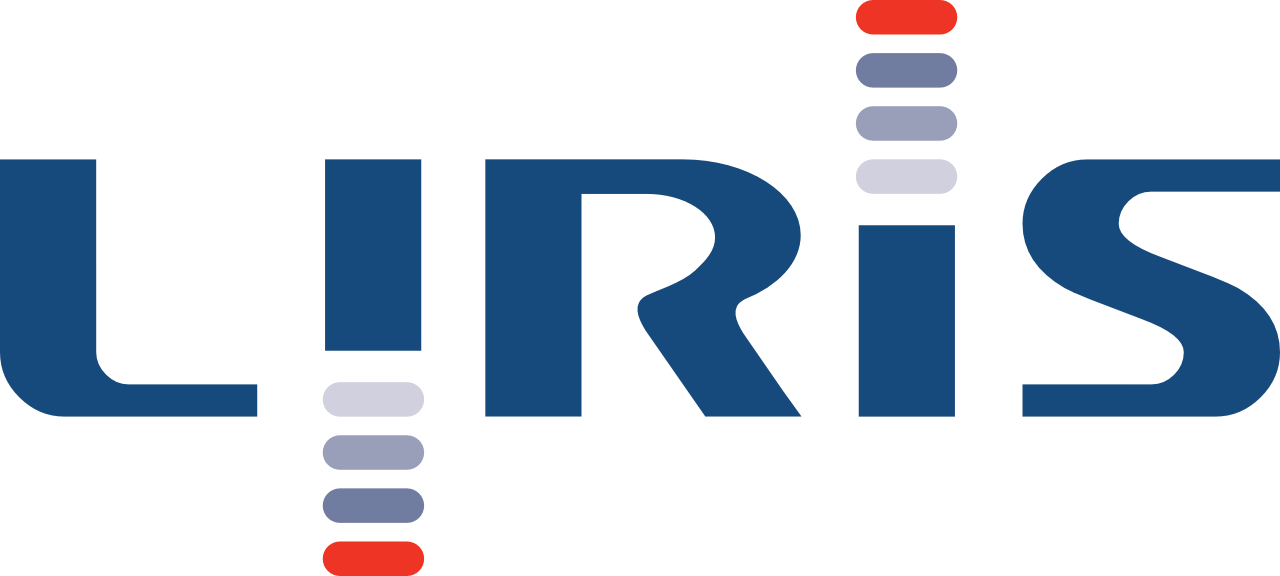
\includegraphics[width=0.25\linewidth, trim= 0cm 0cm 0cm 0cm, clip, valign=c]{Figures/liris.png}
	\label{fig:partners}
\end{figure}

\subsubsection{The validator list}
\label{sec:kiblockchainvalidatorlist}
As mentioned above, limiting the number of validators to a set of selected validators becomes a threat to the security and the fairness of the network. Our solution is a continuously changing list of validators that randomly selects validators out of those eligible, and a new set of validators of equal size are elected at the start of each round. Indeed, when talking about a random election of the validator list, one needs to give theoretical guarantees about the likelihood that the selected set do not present a majority of potentially colluding validators. The higher the number of validators in each round, the lower the chances are that enough colluding nodes are elected. However, this renders the validation round longer, meaning validators must wait longer to get the opportunity to validate blocks.

\textbf{Thesis one:} Continuously renewing the validator list through a random selection process ensures the permanent decentralization of the validation power and a higher incentive for smaller validators to remain part of the process.

\subsubsection{Validator reputation}
\label{sec:kiblockchainvalidatorrep}
In PoS and DPoS systems, a selection metric i.e., the stake and the delegated stake respectively, is used to select the validators. This metric is deterministic and thus, it does not allow any degree of freedom when selecting the validator list, which in turn leads to the centralization problem. The Ki blockchain's PoR consensus algorithm proposes to use an eligibility metric, which as stated before, allows the election of all reliable validators, from which the validator set is randomly selected. In this work, we call this eligibility metric “The Reputation”.

This approach raises multiple challenges. The first is defining what a reliable validator is. We do this by setting a  list of behaviors that define good and bad wallet and validator conduct. In a first iteration, this list will contain well known behaviors such as:

\begin{itemize}
    \item \textbf{Invalid height:} The node has not synchronized the blockchain and is behind the current height.
    \item \textbf{Timeout:} The API/P2P modules of the nodes do not respond.
    \item \textbf{High latency:} The API/P2P modules of the nodes are not responsive.
    \item \textbf{Forks:} The number of times the node has forked from the main blockchain.
    \item \textbf{Too many requests:} The node is emitting too many API requests.
    \item \textbf{Repeat offender:} The number of offences the node has committed.
\end{itemize}

These events can reflect intentional malicious behavior such as attempting a denial of service (DOS) attack, or accidental bad behaviors such as badly configuring the node. In both cases these events impact the performance and the integrity of the network and must be accounted for in the reputation score in order to reflect the reliability of each node.

Once the parameters have been set, we are planning to extend this list by non-destructively probing the network and identifying new behaviors that may be specific to our ecosystem. These behaviors can be used to build a profile for each validator, from which a reputation metric can be computed.

This reputation metric constitutes the second challenge, which can be expressed by the following question: how can the behaviour profile of the validator be translated to a low level numerical value? In other words, suppose that for each validator we build a behaviour profile expressed as a binary vector where 0-bit represents a bad behaviour and 1-bit represents a good behaviour.

To be able to rank validators, a function is required that translate this binary vector into a float based on which the ranking is made. The simple way to do this would be to count the 1-bits in the vector with a higher number representing a more reliable validator. This, however, make the unrealistic supposition that all behaviours are equally important.

In reality, behaviours can be binary, categorical or numerical (continuous and discrete) valued features. One needs to find a way to combine all of them in one float. Indeed, the difficult part is related to finding the weights and the granularity of the features and not really the aggregation function itself. The reputation-based validation process is shown in Figure~\ref{fig:wf}.

\begin{figure}
	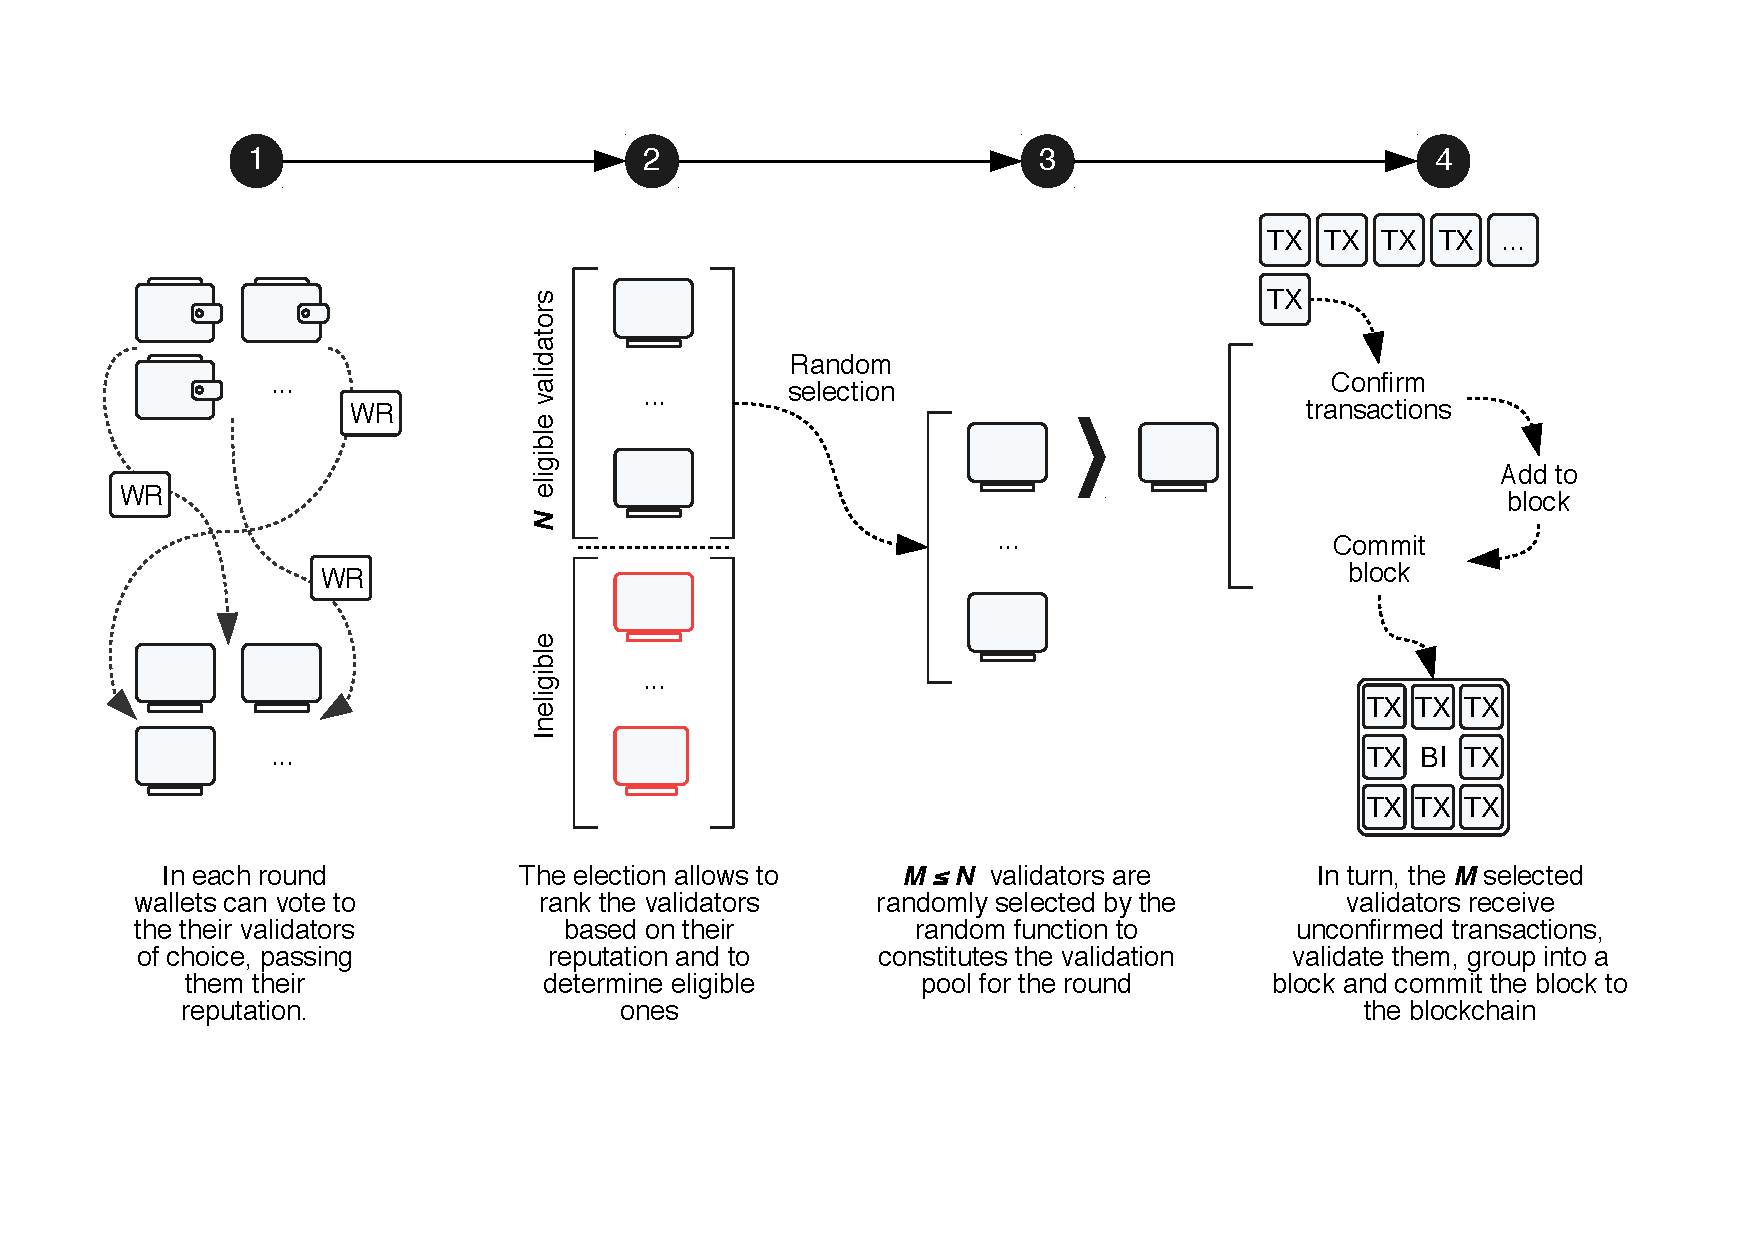
\includegraphics[width=\linewidth, trim= 1cm 3cm 1cm 2cm, clip]{Figures/workflow.pdf}
	\caption{An overview of the block validation workflow in the Ki Blockchain.}
	\label{fig:wf}
\end{figure}

Computing the nodes' and wallets' reputation must fulfill the following requirements:
\begin{itemize}
    \item It needs to punish malicious behaviors.
    \item It needs to penalize negative contributions.
    \item It needs to incentivize positive contributions.
\end{itemize}

\textbf{Thesis two:} Determining the eligibility of the validators based on a behaviour-dependent reputation score, in addition to their stake, guarantees the reliability of the validation process, despite the random selection process of the validators.

\subsubsection{Reputation weighting}
\label{sec:kiblockchainwallets}
Within the Ki blockchain, as staked tokens are within cold wallets, we can use this as an additional factor in calculating validator reputation. The longer tokens have been staked, the greater influence they have on the reputation of that wallet. The structure and attributes of the wallets in the Ki blockchain are shown in Figure~\ref{fig:wallets}.

\begin{figure}
	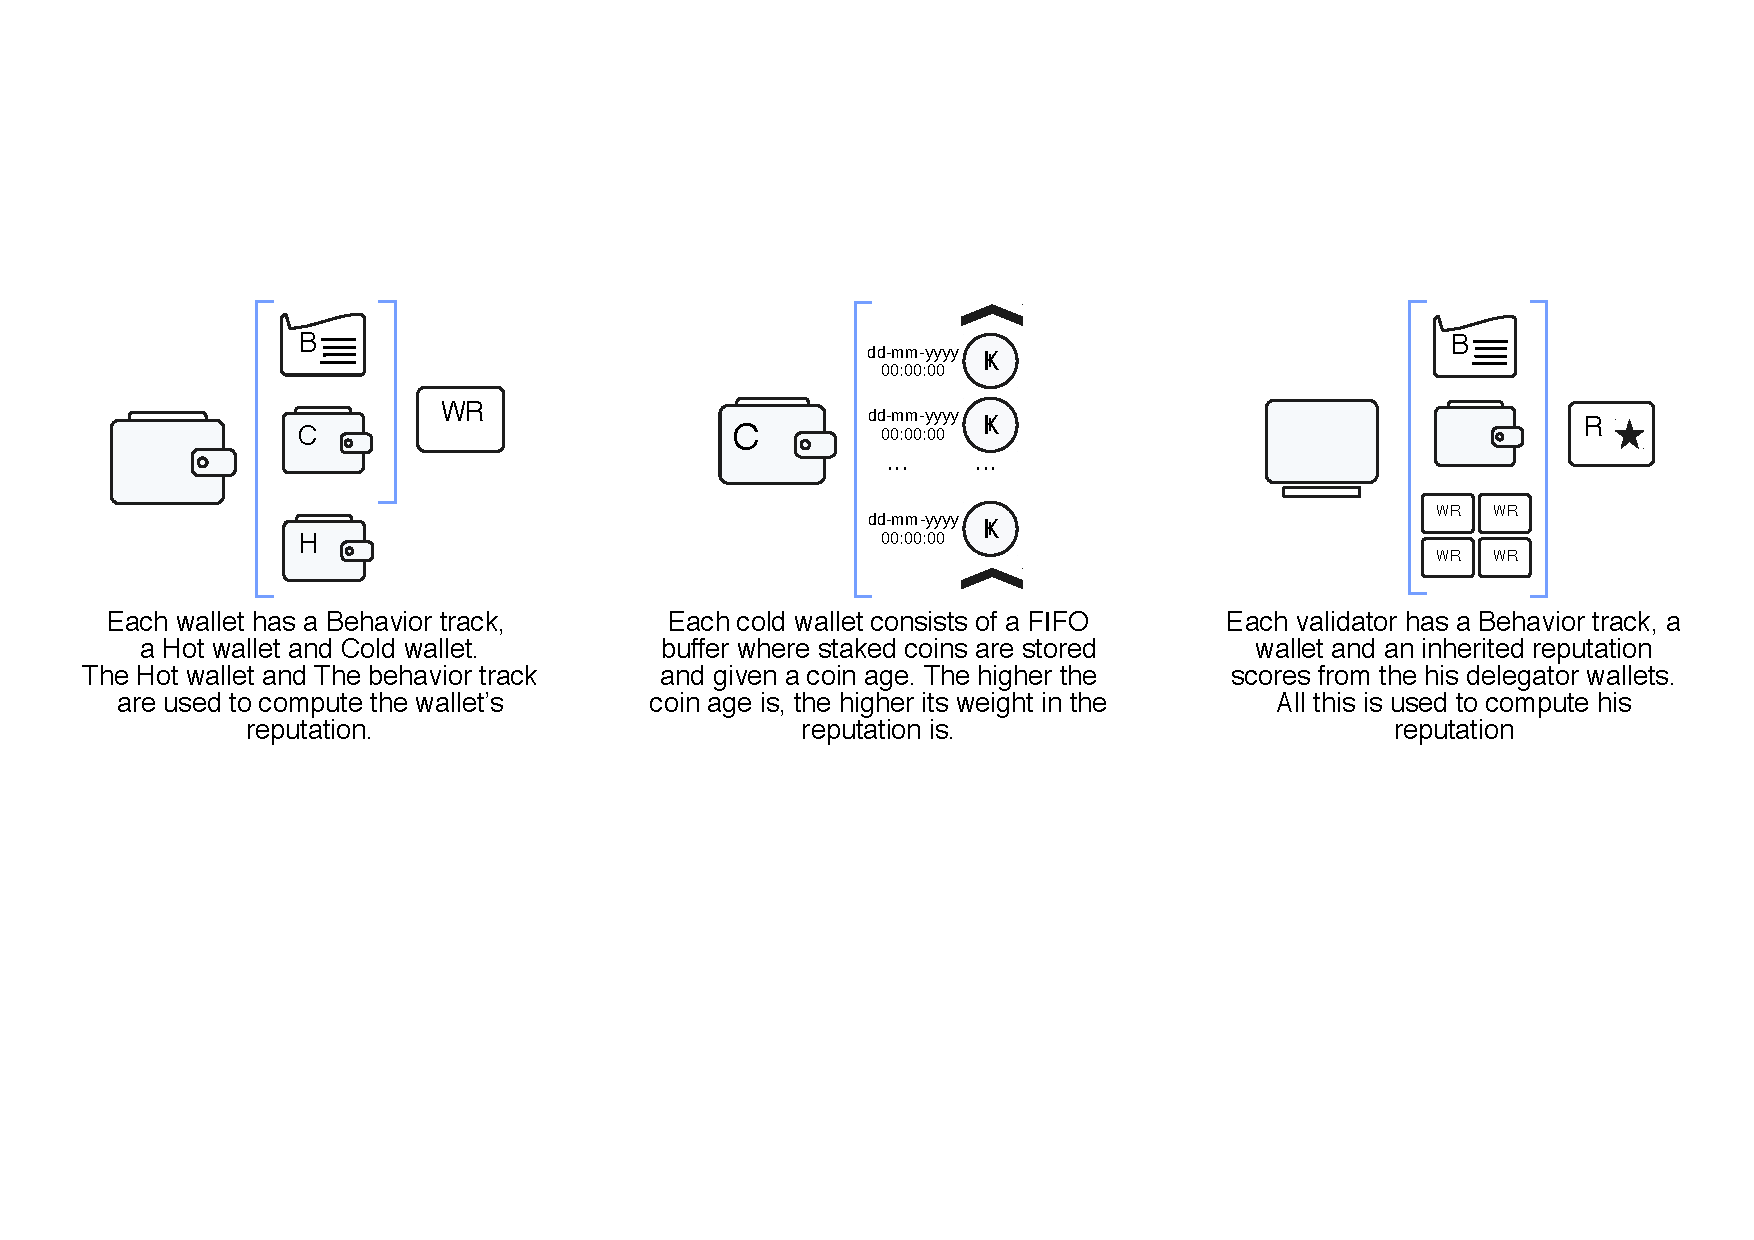
\includegraphics[width=\linewidth, trim= 1cm 8cm 1cm 5cm, clip]{Figures/wallets.pdf}
	\caption{The wallet structure and attributes in the Ki blockchain.}
	\label{fig:wallets}
\end{figure}

\textbf{Thesis three:} Using a cold wallet for staking enables the measuring of staked tokens by their age allowing stake age to be a variable in calculating wallet reputation.

\subsubsection{Dynamic rewards}
\label{sec:kiblockchainreward}
In addition to the distribution of fees from the Ki marketplace,  Ki blockchain will reward validators through inflation of supply, with tokens minted on the creation of every new block distributed to validators. To secure the value of the token, there needs to be tight control over the number of created tokens and their actual usage.

An extreme mechanism that could be used to achieve this value-centric control, is to slash the reward for empty blocks. Rewarding validation of empty blocks creates an inflation that is decoupled from usage of the token. However, whilst it is possible to avoid this “bad” inflation, a zero reward for an empty block can negatively impact validators and their incentives, particularly during the early stages of the network. If these blocks are not paid, there will be no reward for validating these early, empty blocks. Therefore, the reward function must involve both a static and a dynamic reward factor. The first ensures that a minimum reward is paid regardless of the payload of the block (at least during critical periods), and the second ensures that the number of created tokens is controlled and adjusted in relation to the intended yearly inflation rate.

In order to minimize the negative impact of the fixed reward paid for empty blocks, its amount can be optimized by adapting it according to the ratio of empty blocks over the validated ones. Thus, the fixed reward should be adjusted over a period of time. This can be done on a yearly basis through determining the static split of the inflation rate. Eventually this reward will tend to its minimal value\footnote{The static reward never reaches zero. A validator should be guaranteed a minimum payment regardless of the network state.} when this ratio drops below a given threshold. That is when the majority of validated blocks contain transactions, in which case, paying for empty blocks is equivalent to creating negatively contributing tokens. Moreover, the reward paid for an empty block must never be greater than a reward paid for a non-empty one.

The dynamic part of the reward in Ki is computed on a block basis and with regards to the number of transactions per year. That is, the reward paid per block is equal to the total rewards paid for the individual transactions contained in the block.  In other words, the dynamic reward  relies on not only a yearly growth projection, but also the trend of this projection. The dynamic reward adjusts the total reward according to the evolution of the network (from a transaction point of view) and guarantees the balance between a fair reward scheme and a controllable token creation.

Adapting the reward per validating block to the usage of the network allows Ki to master the inflation, and consequently, to maintain the value of the token.

\subsubsection{User privacy}
\label{sec:kiblockchainprivacy}
In the context of blockchain, there are two main facets of node privacy. The first relates to transactions, that is, who initiated a transaction and to whom is it destined. Indeed, preserving the privacy of the nodes (particularly during transactions) may be a requirement for users in the ecosystem (such as service providers) who want to keep their earnings and transactions private. The literature presents a fair amount of strategies that can address this concern with a minimal compromise on the performance and integrity levels. We specifically aim at using two techniques: stealth addresses\cite{CryptoNote} and ring signatures\cite{rivest2001leak}.


\paragraph{Stealth addresses} a.k.a. one time keys, help protect transaction recipient anonymity by achieving transaction unlinkability. That is, a transaction cannot be linked to a given recipient wallet. This is done by creating ephemeral addresses, to which transactions can be sent, and from which only the real recipient can release the funds after the transaction is committed.

\paragraph{Ring signatures} help protect transaction sender's identity. This is achieved by hiding the identity in a crowd of other senders to obfuscate the exact origin of a transaction. The process consists of signing the transaction using the public keys of the crowd members and the private key of one member who actually performs the signature.

The second privacy facet relates to the information needed to trust a node. In the case of the Ki blockchain, this refers to the information required by the Proof of Reputation algorithm to compute the reputation score of a node. The most reliable way of associating a reputation score to a node is knowing the real identity of its owner. This is because it allows verification of the history of the owner and their trustworthiness e.g., by checking their participation behavior in other networks or referring to their public reputation score. Moreover, by giving out their identity, node owners have less interest in behaving maliciously.

Nonetheless, knowing the identity of a node owner violates both their privacy and the promise of a permissionless blockchain. To address this challenge, we consider using nodes' behavior and data publicly available on the network such as it's latency, uptime, forks and so on, as shown in Section 3.2.2. Using these features allows us to build an anonymous profile for each node. A node will then be known and treated based on its behaviour (i.e., it's reputation is computed based on this behaviour) and not on the identity of its owner, since the used features are public and unlinkable to any specific owner.

\subsection{Ki blockchain tools}
\label{sec:kiblockchaintools}
Multiple tools related to the deployment and improvement of the Ki blockchain have already been made publicly available by Ki and other tools will be available according to our development roadmap in the coming weeks. In summary:

\paragraph{Ki devnet:} At the end of December 2018, we deployed the Ki development network (codename: MizuKI) in order to allow the testing of gradual improvements that will be made on the blockchain in a production environment. It is possible for anyone to install and run a devnet relay and validator by following simple steps that can be found at: https://github.com/KiFoundation/ ki-deployer. The Ki devnet launched with 3 seed servers, 51 genesis validators, 5 relays, 5 real validators.

\begin{figure}[!ht]
    \centering
	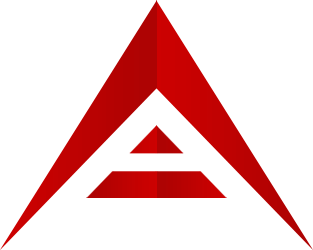
\includegraphics[width=0.3\linewidth, trim= 0cm 0cm 0cm 0cm, clip]{Figures/ark.png}
	\label{fig:ark}
\end{figure}

MizuKI is based on the 2nd version of the ARK core blockchain\footnote{ARK Ecosystem: \url{http://ark.io}}. The ARK ecosystem provides a complete tool bundle that allows for quick deploying of a DPoS based blockchain and can easily configure and use its subjacent tools such as the explorer and the wallets. All this is continuously maintained and improved by an active team and an engaged community. The Ki blockchain uses a fork of the ARK code, in which the DPoS protocol will be substituted by the Proof of Reputation and other functionalities such as the rewarding strategies and wallet scheme will be added. For instance one major enhancement that has been already tested and achieved by Ki's team is to reach, in a test environment, a stable validation throughput of 750 tx/sec with peaks of up to 1000 tx/sec.

Despite the changes, all the currently functioning tools in the ARK ecosystem will easily port to the Ki blockchain, jump-starting the initial network.

\paragraph{Ki explorer:} Transactions, blocks, wallets and validators can be monitored on the Ki explorer, of which the interface is shown in Figure~\ref{fig:explorer}. It is available at: \url{http://blockchain.ki/}

\begin{figure}[h]
	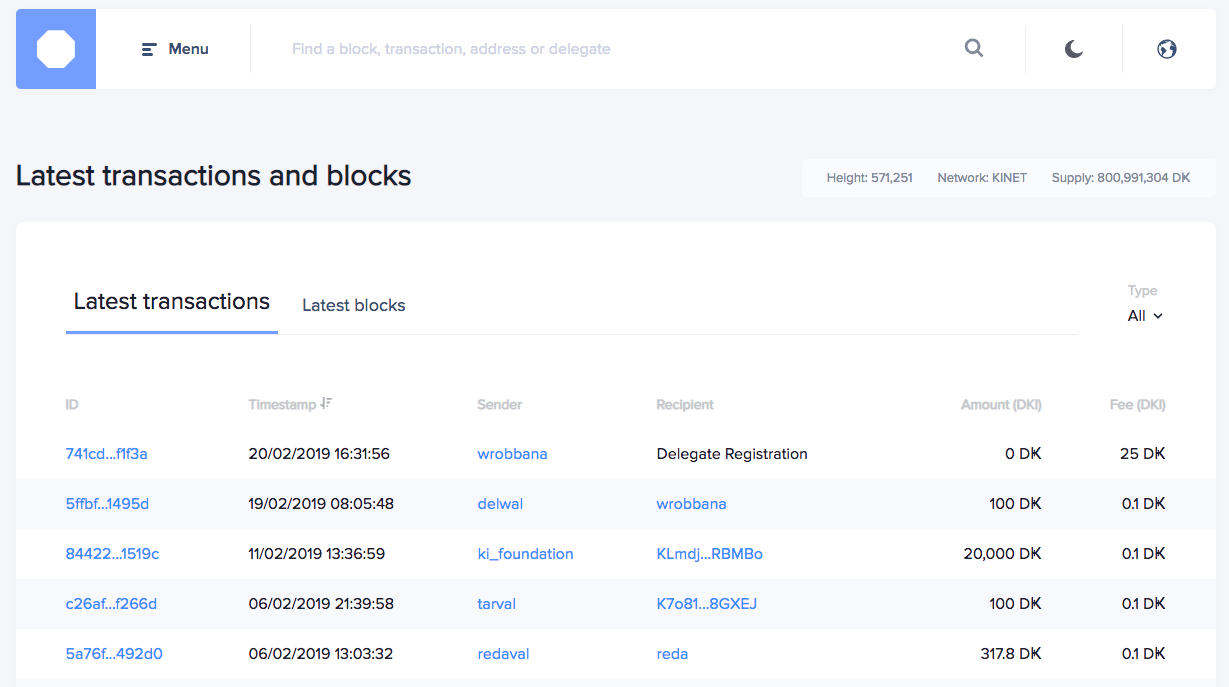
\includegraphics[width=\linewidth, trim= 0cm 0cm 0cm 0cm, clip]{Figures/explorer1}
	\caption{The Ki explorer user interface.}
	\label{fig:explorer}
\end{figure}

\paragraph{Ki wallets} Starting January 2019, the code for building the Ki mobile wallet is available online. A downloadable version is also available on both the Google Play Store and the Apple Application Store. The wallets allow the user to receive and transfer Ki tokens (or DKI tokens on the devnet) as well as to register validators. Multiple views of the mobile wallet interface can be shown in Figure~\ref{fig:walletapp}. The source code of the mobile wallet can be accessed on Github at: \url{https://github.com/KiFoundation/mobile-wallet}

\begin{figure}
	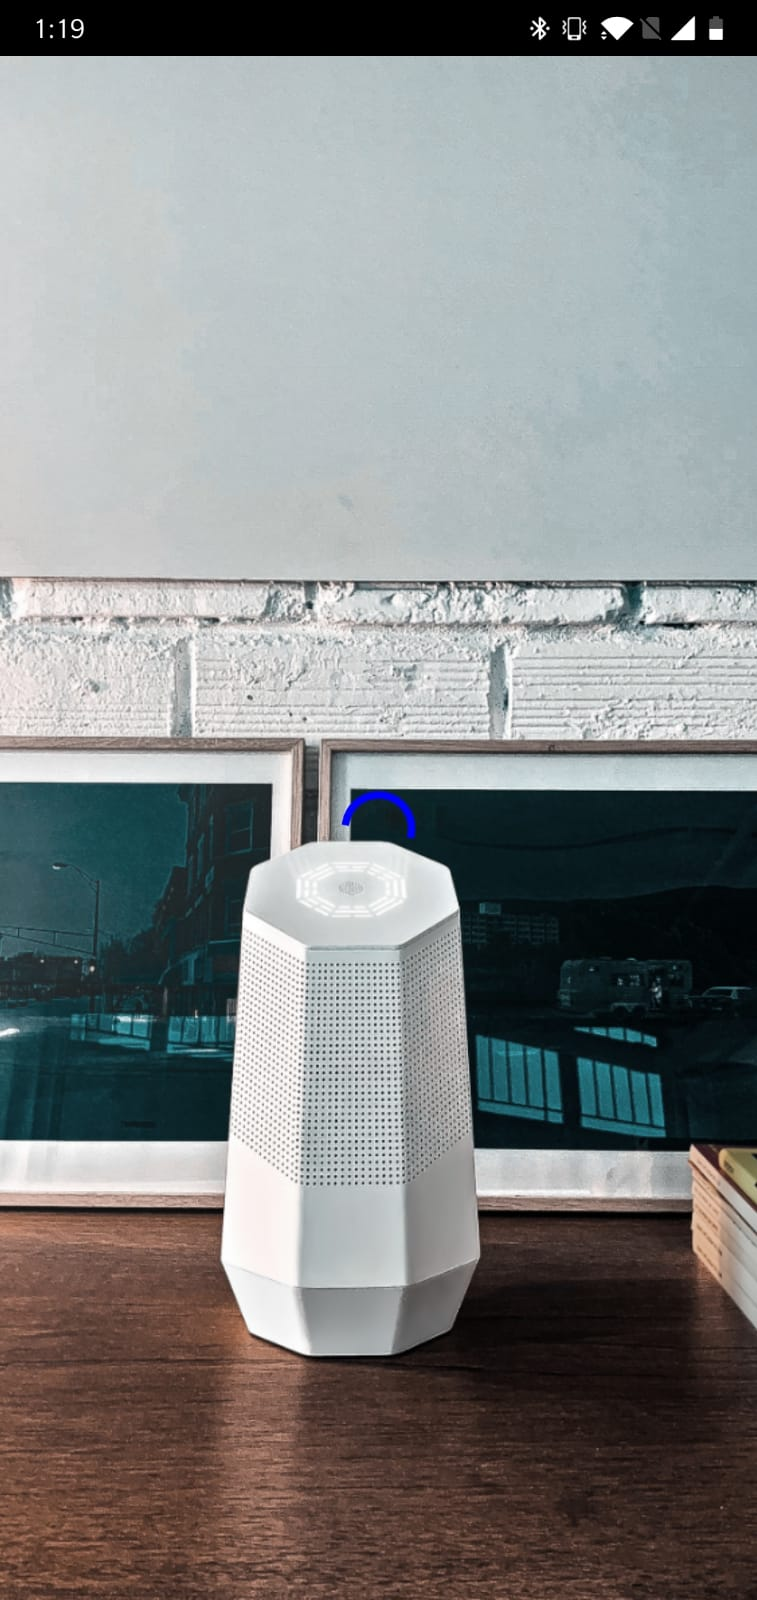
\includegraphics[width=0.32\linewidth, trim= 0cm 0cm 0cm 0cm, clip]{Figures/mw1}
	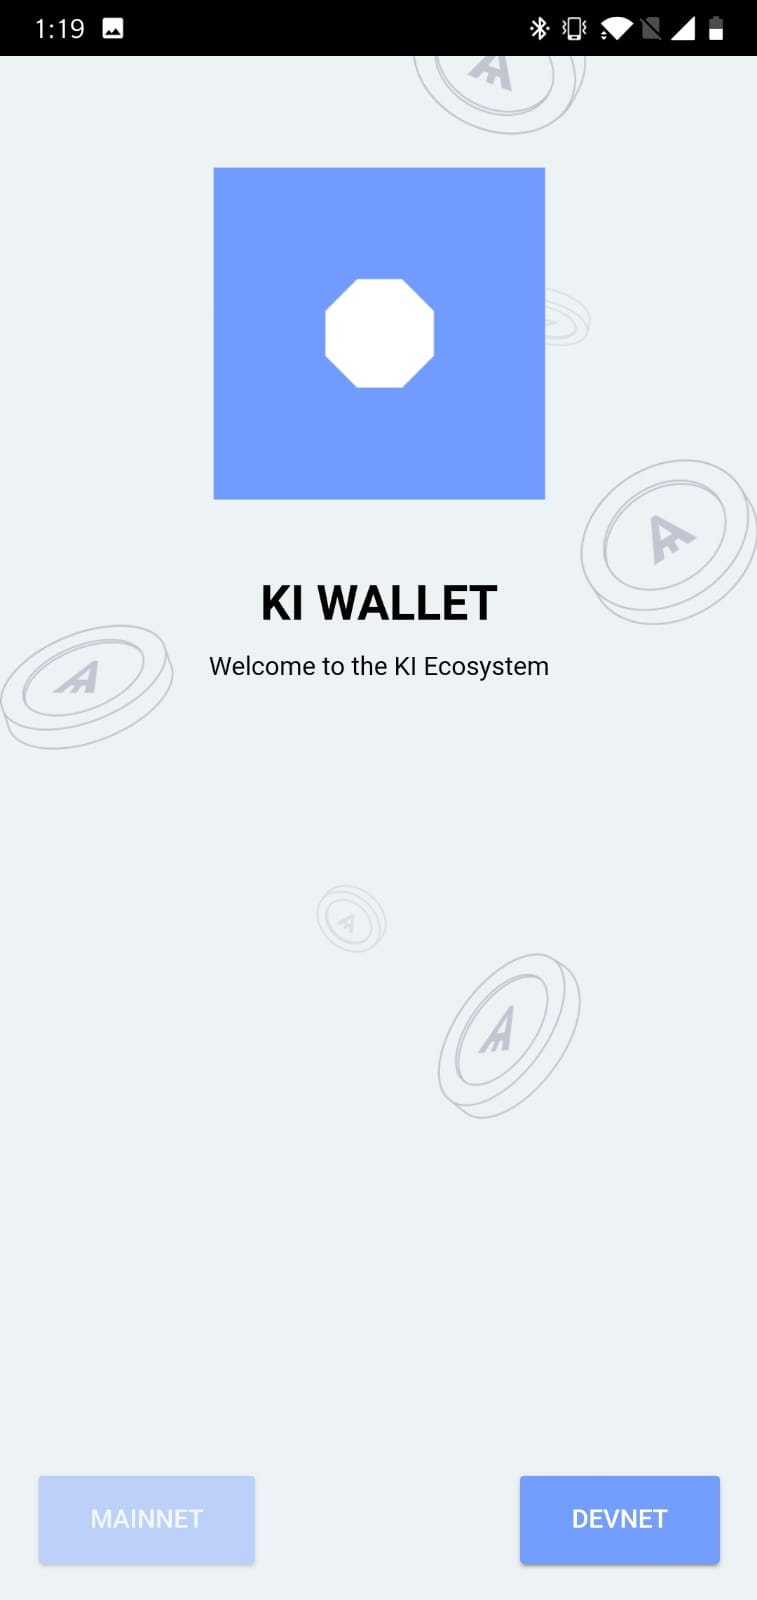
\includegraphics[width=0.32\linewidth, trim= 0cm 0cm 0cm 0cm, clip]{Figures/mw2}
	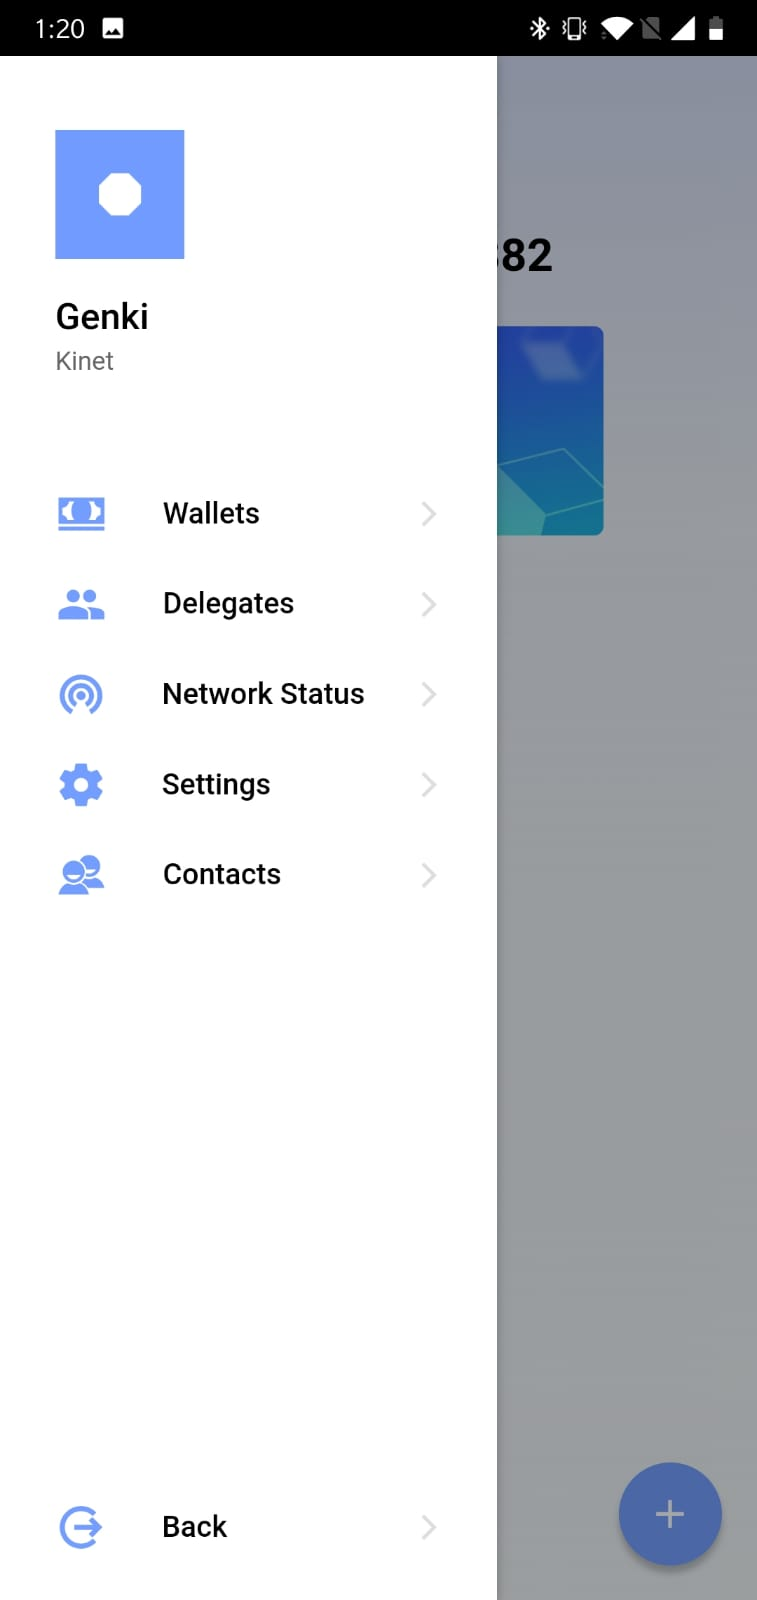
\includegraphics[width=0.32\linewidth, trim= 0cm 0cm 0cm 0cm, clip]{Figures/mw3}
	\caption{The Ki wallet application user interface.}
	\label{fig:walletapp}
\end{figure}

\paragraph{Ki simulator} In contrast with other distributed and peer-to-peer systems, for which well known simulators exist (for example, PeerSim2), there is no simulator adapted to blockchain networks and their scenarios. The Ki foundation plans to accompany the development of the Ki blockchain by the iterative release of the Ki simulator. The Ki simulator aims at giving a better idea on the throughput, stability and security of the network with respect to the protocol parameters such as the number of validators, their behavior, the number of transactions, the reputation measures, and so on. It allows us to simulate situations, which are not - and must not be - easily reproducible in real life. The planned iteration of the simulator will include the following components\footnote{The Ki Simulator can be accessed on github at: \url{https://github.com/KiFoundation/ ki-simulator}}:

\paragraph{Reward simulator} The reward simulator aims to evaluate and compare the stability and consistency of different dynamic and static rewarding schemes on real and synthetic data.

\paragraph{Reputation simulator} The reputation simulator aims at testing the coverage of the behavior aggregation function explained above with regards to the workers' behaviors modeled through configurable scenarios. We plan to build a blockchain specific language on top of the RACOON\cite{lenacota2015} and SEINE simulators\cite{cota2017analysing} to extend its support to blockchain related selfish and malicious behavior.

\paragraph{Performance simulator} The performance simulator aims at evaluating the scalability of the blockchain from the throughput (tx/sec) perspective. This is to study the impact of removing the size limit of the validator list, the random selection and the reputation computation on the network performance.\\

To date, a prototype of the reward simulator has been implemented in Python. The current version is constituted by the following modules:

\begin{description}
    \item[a. The data generator] This module enables the following tasks: (i) loading and formatting transaction data from a data file, (ii) generating transaction data from a preset distribution configuration (iii)  generating a set of validators with their relative stakes from a preset distribution configuration and (iv) distributing the validation spots over the generated validators based on a preset strategy.

    \item[b. The forecasting module] It allows us to make predictions on the number of transaction based on historical data, which in turn is based on known models such as the "Autoregressive integrated moving average" (ARIMA) \cite{saboia1977autoregressive}.

    \item[c. The reward calculator] This  allows us to compute the reward based on 4 models: (i) transaction based reward, (ii) block based reward, (iii) hybrid reward and (iv) transfer based reward (Ki's model). Besides this, it allows us to compute the individual reward of each validator based on their validation spots.
\end{description}

\subsection{Ki blockchain roadmap}
\label{sec:kiblockchainroad}
It is clear from the previous discussions that the technical challenges ahead of Ki are interdependent. Moreover, it is clear that besides the needed implementation and development effort, an upstream theoretical effort is mandatory. The dependency and research aspects that are more challenging, imply gradual and interlaced work. That is, at each milestone we will be fixing, as much as it is logically possible, all the elements except the one we are dealing with at that moment. The roadmap in Figure~\ref{fig:roadmap} depicts this process and shows how the task will be distributed over the upcoming year, with the ultimate goal being to launch a testnet that fully supports the PoR consensus protocol by the end of December 2019.
\begin{figure}[h]
	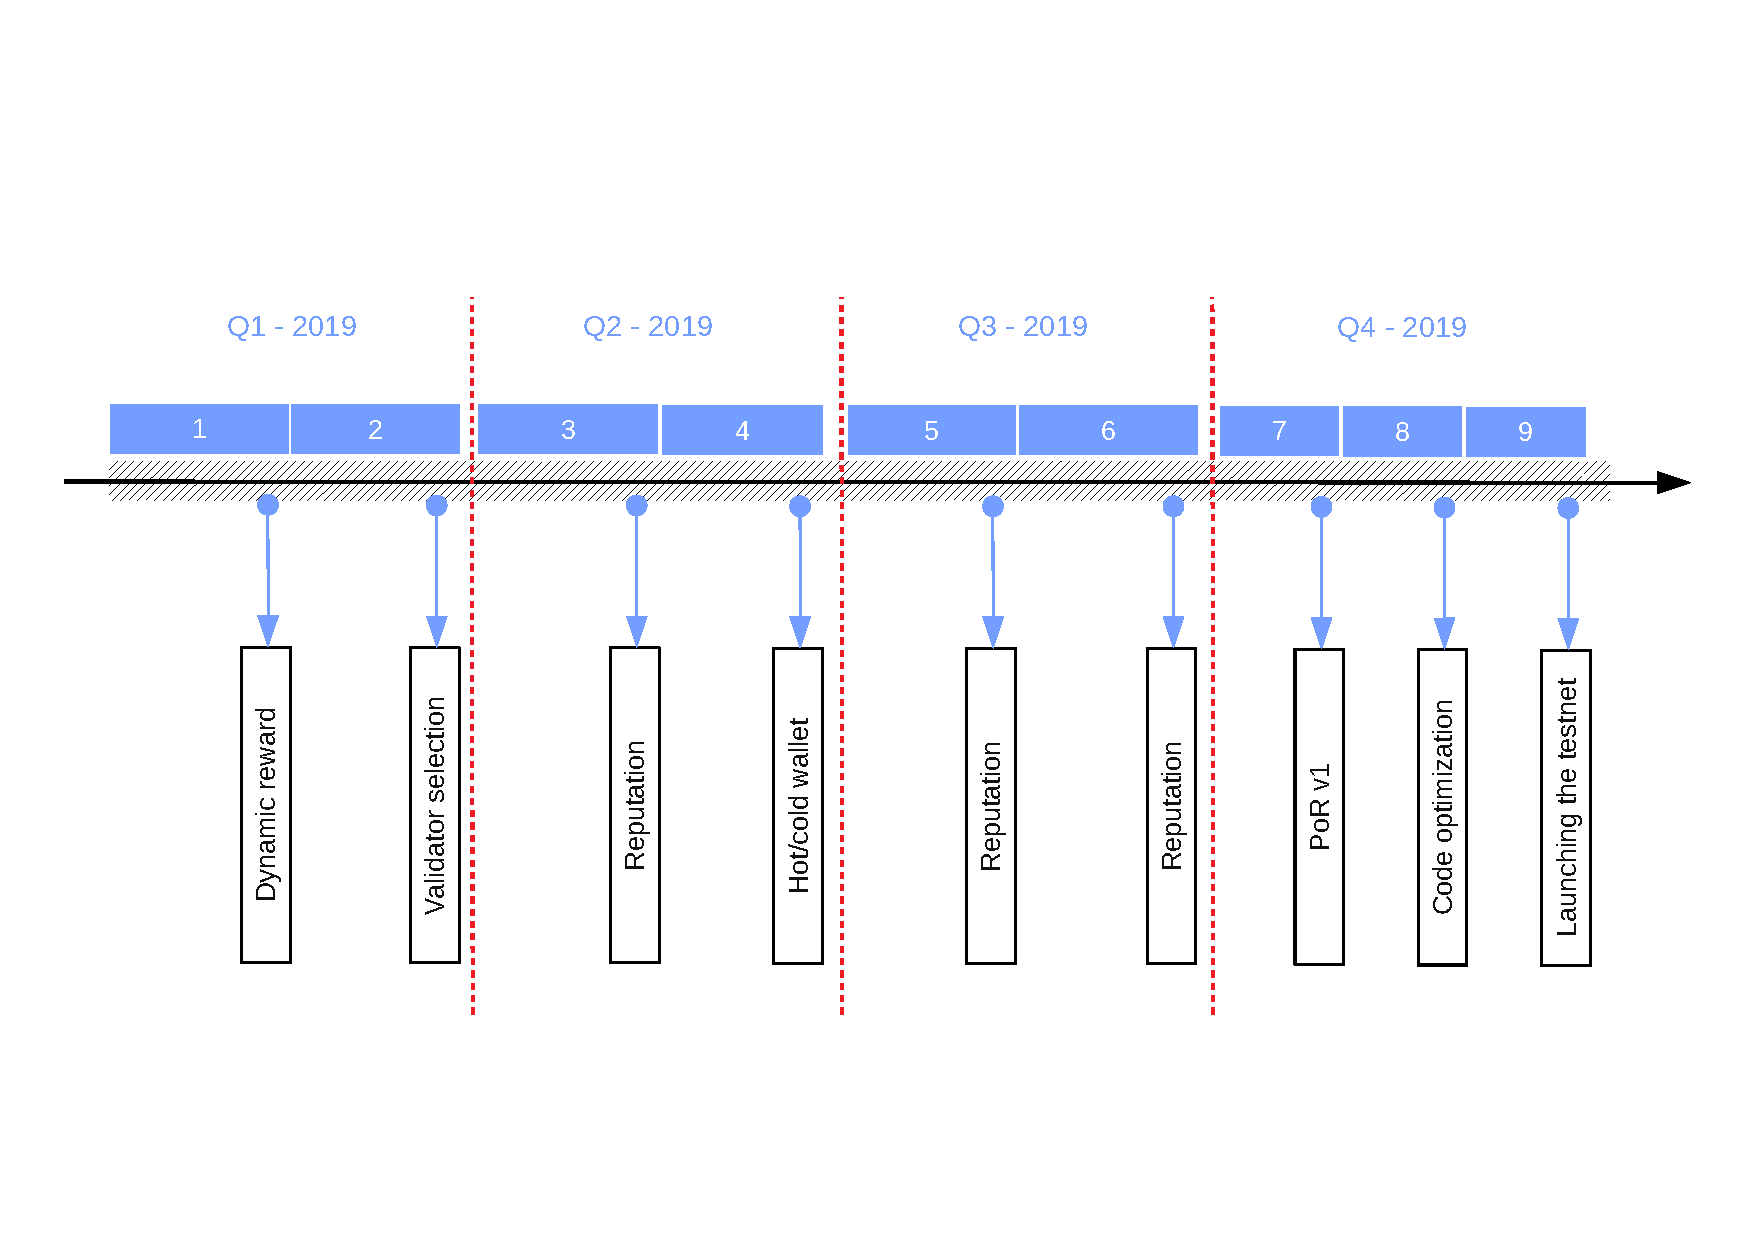
\includegraphics[width=\linewidth, trim= 1cm 3cm 1cm 3.5cm, clip]{Figures/Roadmap_f.pdf}
	\caption{An overview on the research and implementation roadmap of the Ki blockchain.}
	\label{fig:roadmap}
\end{figure}
\section{The Ki device}
\label{sec:kidevice}
Ki's homepod enables owners of untapped IT assets to monetize their spare capacity, in a similar way to how AirBnB enables homeowners to monetize spare rooms within their own households. The Ki device exists to protect its owner's digital sovereignty, while allowing them to monetize their untapped digital assets. On a larger scale, the Ki device can be seen not only as the hub of a smart home ecosystem, but also as a core component of tomorrow's smart city, managing its inhabitants' IT assets as cleverly as a smart grid can manage a city's energy [3]. To achieve such a vision, Ki needs to address different challenges:

\begin{itemize}
	\item Unify heterogeneous wireless communication technologies to make Ki's Homepod a hub to all the digital assets located on its owner's local area network.
	\item Give true digital sovereignty to its owner over their LAN, by letting them monetize their IT assets as they wish, without any central control, not even Ki's.
	\item Ensure the end user's privacy.
\end{itemize}

Addressing these issues in a comprehensive and effective way led us to create the Ki device: a smartspeaker that is also a powerful network hub, which includes all the needed components and software to communicate wirelessly, manage applications, and share resources, all the while ensuring security and privacy for its users. Figure \ref{fig:domo} depicts the technical specifications of the Ki device.
\begin{figure}[!ht]
\centering
	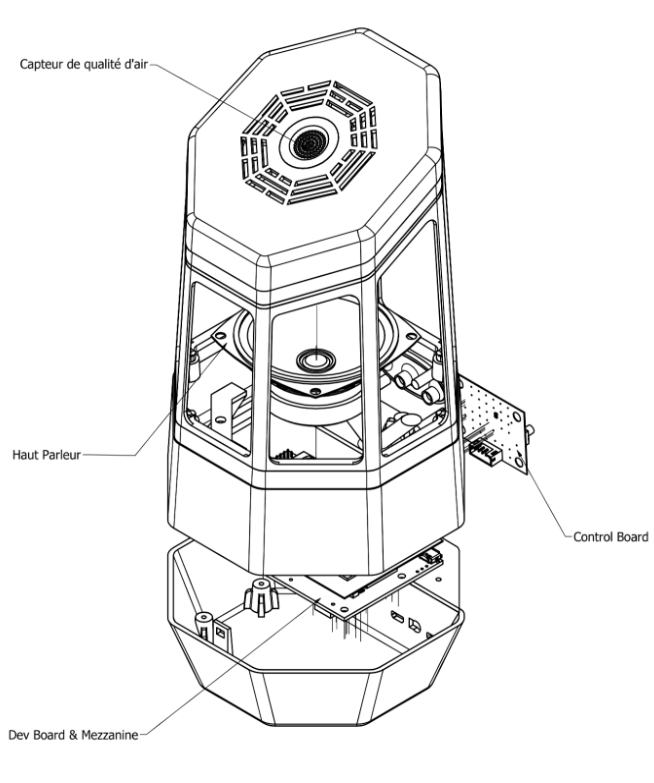
\includegraphics[width=0.4\linewidth, trim= 0cm 0cm 0cm 0cm, clip]{Figures/domoE.png}
	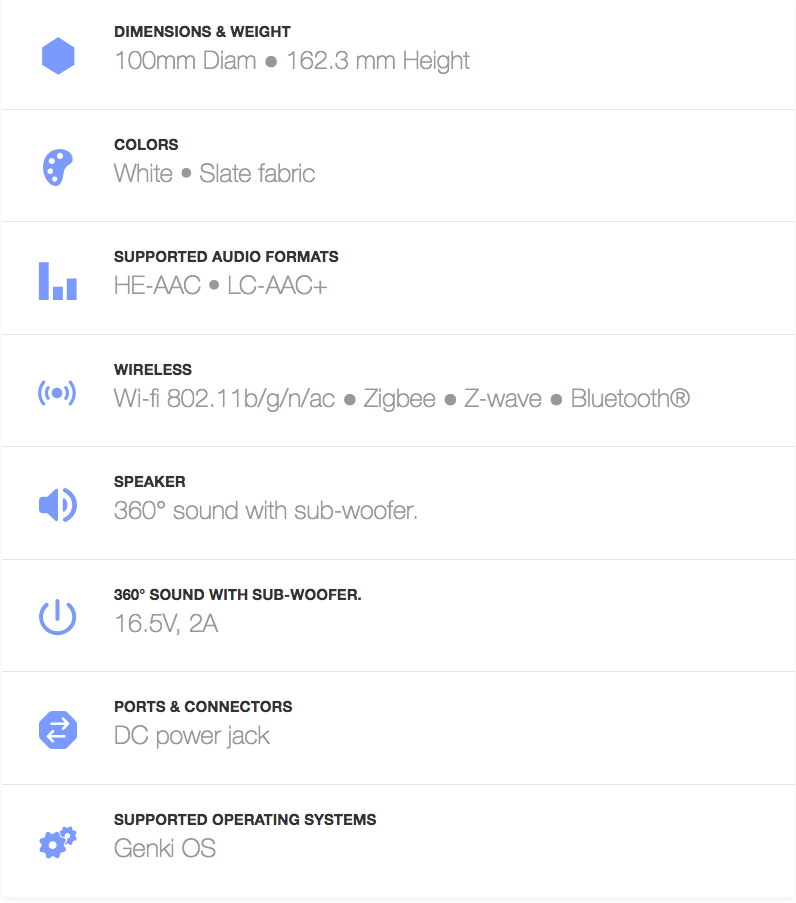
\includegraphics[width=0.4\linewidth, trim= 0cm 0cm 0cm 0cm, clip]{Figures/domoS.png}
	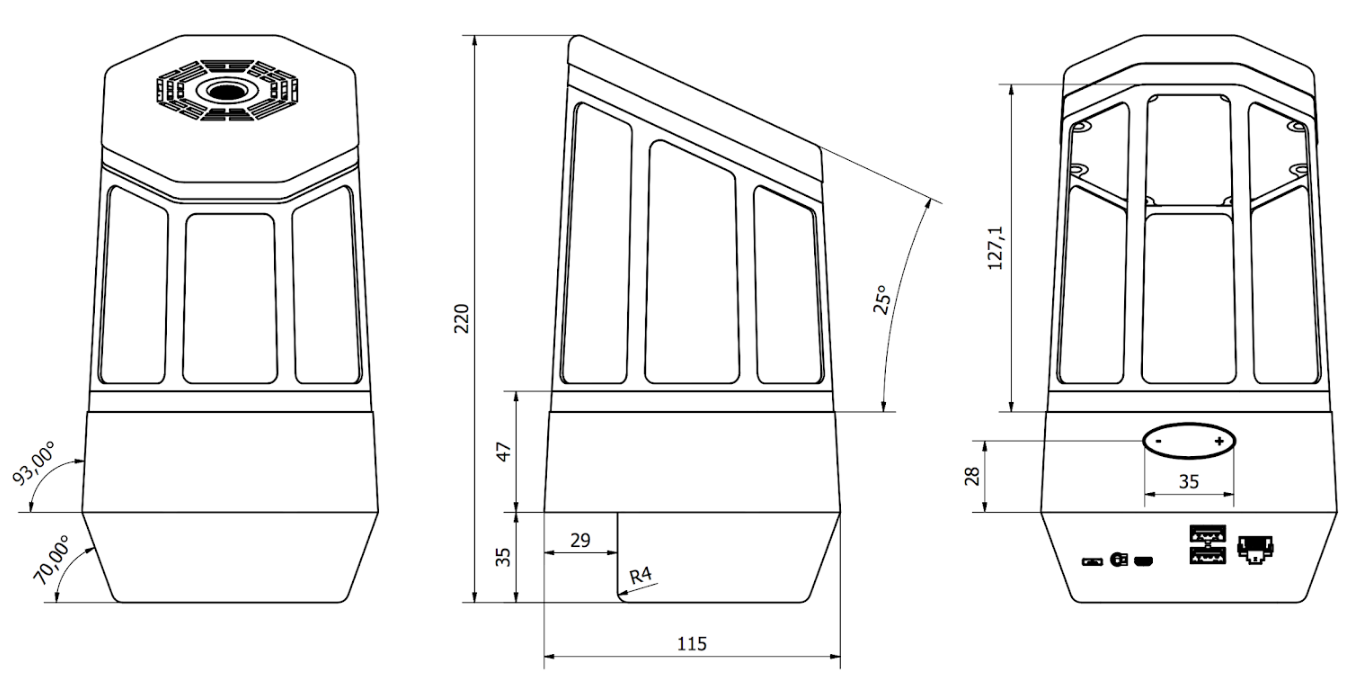
\includegraphics[width=0.8\linewidth, trim= 0cm 0cm 0cm 0cm, clip]{Figures/domoB.png}
	\caption{The Ki device specifications.}
	\label{fig:domo}
\end{figure}

\subsection{A privacy-first approach}
\label{sec:kideviceprivacy}
A privacy-centric approach drives the integration of privacy-friendly technologies in the Ki device, such as its voice platform that runs locally, ensuring that its users' conversations aren't uploaded to a cloud-based system. This means that they remain private at all times. Ki's users' voices, which are a critical biometric footprint, are not shared with anybody. Every technology built for the Ki network is done with a “privacy-by-design” approach, and every algorithm that uses user data, runs locally and securely. Privacy is a fundamental part of Ki's approach to building a smart speaker: we consider it a fundamental right. Furthermore, other smart home devices are simply a speaker and a microphone. They cannot support a network or the new decentralized internet.

% \begin{figure}[!ht]
% 	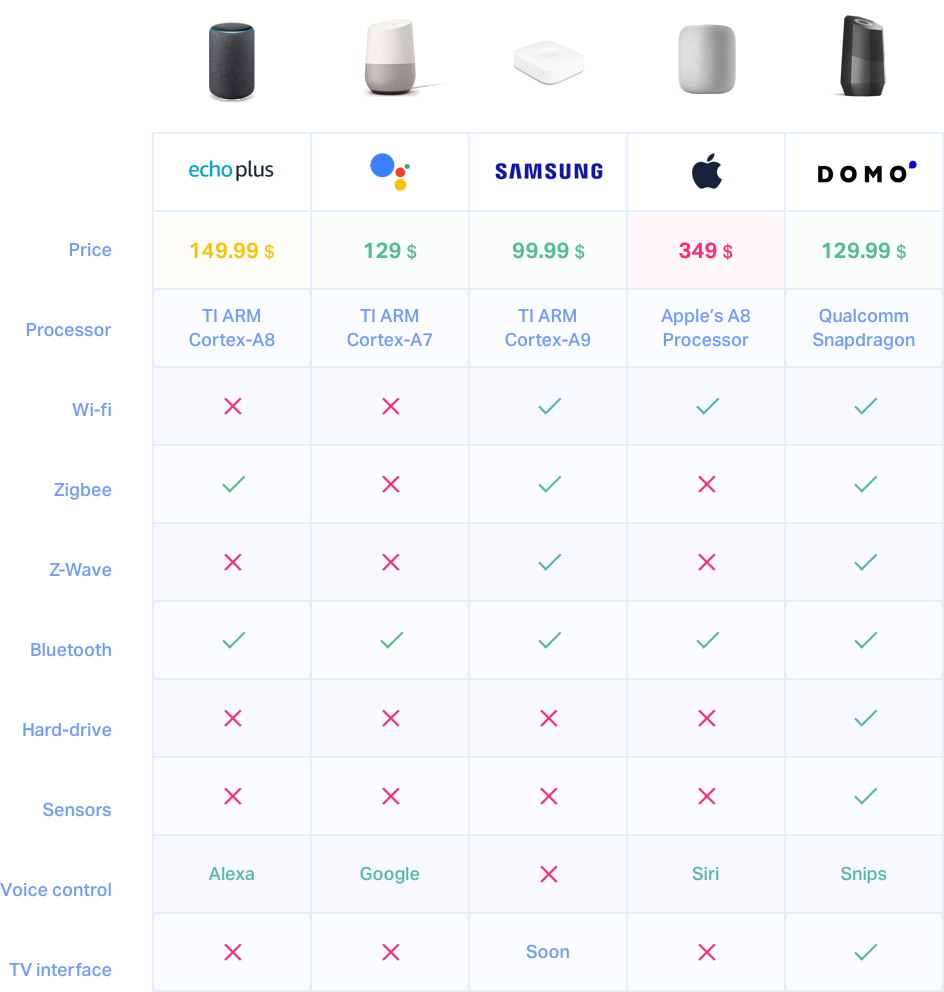
\includegraphics[width=\linewidth, trim= 0cm 0cm 0cm 0cm, clip]{Figures/domoD.png}
% 	\caption{Smart speaker competition scorecard.}
% 	\label{fig:smart}
% \end{figure}

The Ki Foundation has built a home device that utilizes a new Operating System based on AOSP, holding libraries supporting a blockchain-based, decentralized application store (the dApp Store). None of the components of the Ki ecosystem: the Ki device, the Ki operating system, the Ki blockchain or the Ki dApp store, can ever be leveraged to listen, manipulate or monetize its user's personal data.

Unlike existing smartspeaker devices that simply have a microphone and a speaker, Ki's device (fig. below) is a real computer, equipped with powerful processors, an SSD storage and multiple sensors. As such, every Ki device can be setup as a validator node in the Ki blockchain, contributing to the operation, maintenance and governance of its ecosystem. The Ki device is equipped with a loud speaker and smart sensors that can track energy usage, temperature, air quality and humidity, each functionality is carried out without transferring such data outside of the home.

The Ki device provides Wifi internet through two different channels: 1) an Ethernet plug, or 2) eSIM solution service that enables data traffic in more than 200 destinations world-wide. The eSIM provides a fallback connectivity solution in case the landline internet is cut. Very significantly, this means that in the future, the Ki ecosystem will be able to provide local internet to devices all around the world: connecting people whilst protecting privacy.



\subsection{Building resiliency and security}
\label{sec:kidevicesecurity}
Relying on a centralized cloud-based technology to supply essential internet services will inevitably run into the "single point of failure'' problem [8], risking, at a minimum, a temporary disruption of your access to internet-based services. With Ki, users do not have to rely on a unique service provider or hardware provider to benefit from essential internet services and users therefore become resilient to such severance.

No centralized authority should be a point of failure for any internet users, preventing them from accessing essential services or their data, or worse, failing to keep their data safe.


\section{The Ki ecosystem }
\label{sec:kiecosystem}


\subsection{Stakeholders}
\label{sec:kiecosystemstakeholder}
The Ki ecosystem is made up of three kinds of players, each with a distinct role in the proper and efficient functioning of the network.

\paragraph{Validators:} A validator is a fully synchronized node, willing to stake it's tokens (or part of its tokens) to secure the network (i.e., willing to participate in the consensus protocol). A validator is paid in Ki tokens for their participation. These validators contribute to the consensus by broadcasting votes cryptographically signed by each validator, using their private key. Validator candidates can stake their own Ki tokens or have tokens "delegated'' to them by delegators.


The Ki blockchain can have an unlimited number of validator candidates due to its PoR consensus algorithm. Validators and their delegators will earn a dynamic amount of Ki tokens, depending on the number of daily transactions witnessed on the system. All of the fees charged to run the Ki marketplace are shared amongst the validators and delegators who processed the transactions in question, and none go to Ki. This is because Ki is a foundation with no equity and no desire to extract rent from the participants in the Ki ecosystem. Ki tokens are the only way in which someone can participate in the growth of the Ki ecosystem.

There will also never be any transaction fees for using the Ki network itself, although a validator will be able to charge a commission on the tokens forwarded to their delegators as an incentive for running a full node. If a validator misbehaves, its reputation is affected, and its staked Ki (including delegated tokens) can be slashed. The penalty depends on the severity of the violation.

\paragraph{Delegators:} A delegator is a node that does not synchronize the full blockchain, but which lends part of its stake to help a validator increase its stake; the validator then redistributes the corresponding share of its reward to the delegator. In this way, a delegator can also take part in securing the network and be rewarded proportionally to the amount of tokens they are willing to stake. If a validator's stake is slashed due to an invalid behavior, the delegator's share of the stake is slashed as well. As a result, the delegator shares this risk and must delegate wisely.

\paragraph{Service providers and developers:} By requiring apps to be installed through App Stores, under the control of those managing the operating systems, a choke point was created. Since most people rely on Apple or Android operating systems for their devices, these companies have gained huge leverage on the flows of information. The Ki ecosystem is underpinned by the Ki blockchain, bootstrapped by the Ki device and will have the dApp Store at its core. The dApp store will be an open platform using reputation and staking mechanisms to allow third-party software developers to reach new markets, and use decentralized resources to offer innovative services on a secure and trustless basis.


By embracing decentralization, developers won't need a third party to manage transactions, thereby avoiding transaction fees. The dApp store will manage the reputations of the developers and service providers selling to consumers using certain of the techniques incorporated in the PoR algorithm. Governance of the dApp Store will eventually be completely delegated to the open source code developed by the Ki foundation and the votes of the holders of Ki tokens. Certain stakes of Ki tokens will be required to sell services and develop applications for sale in the dApp Store. A service provider can provide value to end users (e.g. selling services or renting out it's unused hardware resources or bandwidth through third party Web3 applications) and get paid in Ki tokens for the value they provide.

Device owners: By acquiring a Ki, you can also become a full actor in the Ki blockchain: by staking Kis as a validator and by providing the devices' storage and processing power to maintain and secure the blockchain.

IoT fleet owners will also be able to join the network and offer their computational power, network and storage for Ki tokens. For example, public WiFi providers, connected hard drives owners, router manufacturers, etc. could all provide computing, storage and validation services. Examples of other devices that could become part of the Ki ecosystem include: public WiFi providers, connected hard drives owners, router manufacturers, etc.


\subsection{Bringing wireless communications together}
\label{sec:kiecosystemwireless}
Big tech companies have a natural tendency to impose proprietary protocols to enforce their monopoly. In the IoT emerging market, the same trend has been observed across all actors: from Amazon's Zigbee routing to Samsung's z-wave routing, and throughout other wireless technologies such as Sigfox and Lora. This led us to create an agnostic technological layer, merging all systems and acting as a conductor, orchestrating all communications with a fully open protocol that shares value for all - rather than extracting value for the few.

While the world is currently embracing various home-connected hardware, their use and interaction is still limited to basic tasks, mostly due to a lack of a coherent layer unifying communication protocols, application stores and resilient services that are open to the broader software development community. The Ki device aims to become the cornerstone of a new internet, Web3.0. It is a decentralized infrastructure that provides the ability to deploy a truly decentralized, fair and transparent ecosystem.

\begin{figure}[!ht]
	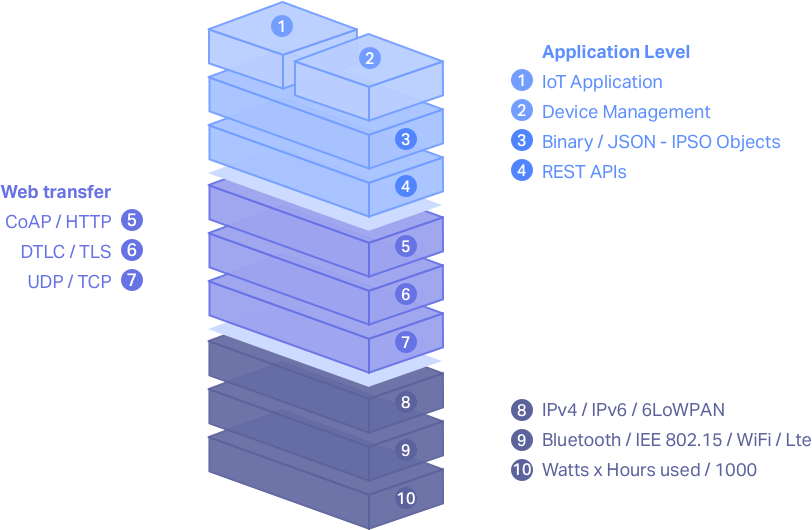
\includegraphics[width=\linewidth, trim= 0cm 0cm 0cm 0cm, clip]{Figures/iot.png}
	\caption{Layers of value and service in the IoT world.}
	\label{fig:iot}
\end{figure}

\subsection{Enabling a global decentralized mobile network}
\label{sec:kiecosystemmobile}
To support the new decentralized internet, Web3, we also need to distribute and decentralize the stack that provides the computing power, energy, bandwidth and storage to run it. With the explosive growth of IoT and other decentralized applications, we see another compelling need to support the process of local compute, store and communication. With the more demanding requirements of autonomous vehicles and ever smarter IoT devices, the conventional cloud model of having to rely on remote centralized computing resource is no longer feasible to support billions of connected devices requiring near real-time latency at all times.

One example of how Ki can support a seismic shift away from the concentration of power by centralized systems, is how Ki proposes to ultimately enable a new kind of mobile operator, a real alternative to the large and powerful mobile network operators of today. Each Ki device is equipped with built-in wireless protocols including Zigbee, Z-Wave, Bluetooth 4.0+ and the eponymous Wi-Fi. A network of Ki devices can readily create a local meshed network using such wireless protocols. Ki is currently working with a global partner to build the capability to allow any smartphone to seamlessly use the closest Ki meshed network for mobile voice and data communication. The Ki blockchain would be leveraged to pay for the bandwidth usage. Each participating Ki device owner would receive Kis as payment for the used bandwidth and all other fees would be distributed in Ki (or via Ki's fiat onramp/offramp) to the technology provider of the virtualized phone number and soft-switch technology as well as the validators and delegators who secure the Ki blockchain and process the transaction.

Using a blockchain-based alternative to the identification of mobile devices would allow efficient but private access to Ki's proposed decentralized mobile network on a global scale. To arrange for payment for access to all mobile connectivity, ordinarily, it would be necessary to identify a device every time it enters a new network territory. While this would appear to cause issues for a decentralized service, since each base station would be a node of the Ki blockchain, the connecting device could be authenticated quickly by sending its public key to the network to identify the device. This action would be carried out by the Ki wallet, which would broadcast its public key generated from the private key, which is stored securely on the device. Neither the carrier nor any other third party would need to know nor have access to the private key in question. This concept, the ``KiSIM'' solution, allows for the identification of registered subscribers using the local meshed network but protects each subscriber's personal information using public-private key cryptography.
\begin{figure}[!ht]
\centering
	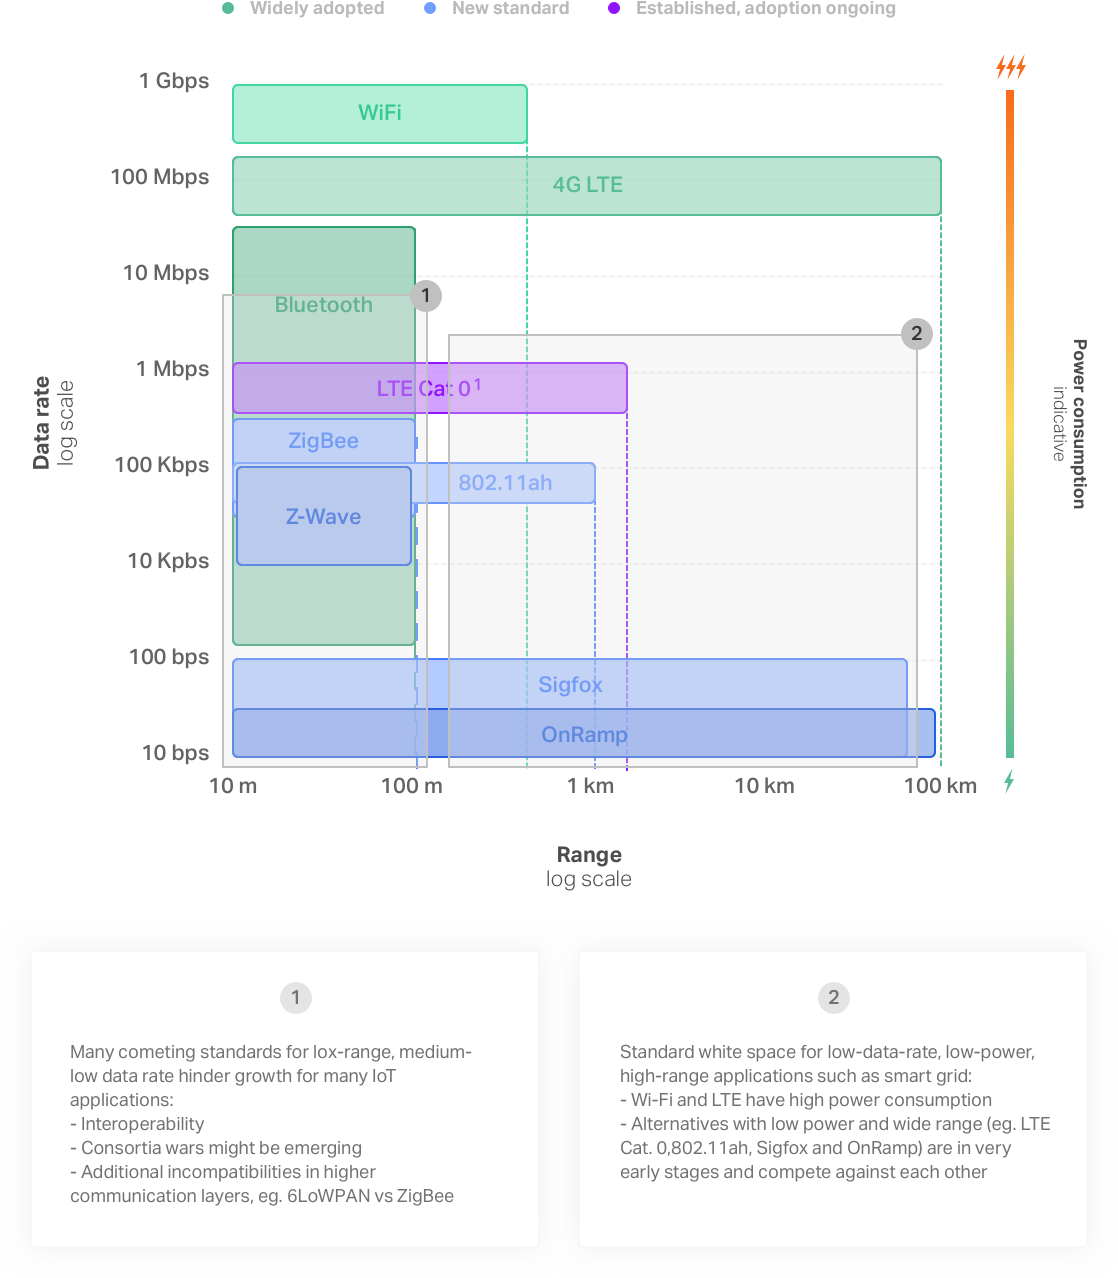
\includegraphics[width=0.9\linewidth, trim= 0cm 0cm 0cm 0cm, clip]{Figures/wireless.png}
	\caption{Range and data rate of the existing wireless communication technologies.}
	\label{fig:wireless}
\end{figure}
Looking at how a meshed mobile network could work in a major urban area like Paris, it is necessary to make certain assumptions around the required connectivity and bandwidth needed to support such a system based on the current technical specifications of the Ki device and the average calls per mobile advice in the Paris region as per March 2019. The first assumption is that each Ki device can support 10 to 15 active phone connections, based on its average bandwidth, processing power and storage. The second is that the network would be required to deal with 8.7 billion phone calls a day of approximately 3.6 minutes each, for a total of 30 billion minutes. These numbers estimate that 5,000 active Ki devices could handle such a load, but for security and reasons of failsafe redundancy, we would suggest doubling the number of devices required. Based on these assumptions, 10,000 active Ki devices could support a decentralized mobile network in a city with a population and landmass of Paris. The capital expenditure required to build such a network would be 5\% (\$20m v \$1.2m for 10,000 devices) of the classic cell-tower alternative and approximately 1\% of the operating expenditure (maintenance and electricity costs of \$80m v \$100k, i.e. \$10 per Ki device).

Looking at Ki's end-vision, beginning with 500,000 devices, the Ki network could support over 10\% of the global demand for internet bandwidth,  provided in a distributed, decentralized and secure fashion, and coordinated by the Ki blockchain.




\subsection{The Ki Token}
\label{sec:kiecosystemtoken}
Within the Ki network the native Ki token is used to facilitate all services and transactions on the network. It also provides the holder with the ability to validate, delegate to other validators and to vote on Ki network proposals. The Ki token forms a pivotal role in maintaining the security of the Ki blockchain and rewarding validators for securing the network.


The Ki token serves a number of roles within the Ki ecosystem:

\begin{itemize}
\item As a unit of account within the Ki network
\item As a means of transacting within the Ki blockchain and Ki dApp store
\item As a means of transferring value for unused resources and third party services
\item As a means of incentivizing validators and delegators to secure the network
\item As a means of transferring marketplace transaction fees in the Ki decentralized dApp store: all fees are shared among the actors of the ecosystem: such as customers, app developers and token holders participating as validators and delegators within the network and hotel owners.
\item As a means of building reputation within the Ki's PoR consensus.
\end{itemize}

The Ki tokens' initial supply has been set to 800 million tokens, but is not fixed. The Ki token has an inflationary policy to compensate validators through newly issued Ki tokens. Each Ki token staked is time-stamped with the date of the staking, which provides its staker a higher validator weight the older the timestamp.

The Ki device brings valuable users to the Ki marketplace through the hospitality market. Further, a distributed network of devices (i.e. nodes) can share their spare storage, computing power, and bandwidth on a coordinated basis using the Ki marketplace and token as the medium of exchange.


\section{Governance}
\textit{``Governance: the process by which we attempt to establish (and maintain/revoke) the legitimacy of decisions, decision-making processes, and related governance norms/expectations''. \href{https://twitter.com/VladZamfir/status/974026020234948608}{Vlad Zamfir}}


Governance is the most challenging issue to get right in a decentralized system. We can conceive of many ways to establish the legitimacy of decisions. In some contexts, voting can play a critical role. In others, it's not needed. However when decisions affecting the network are made, they must make sure that all stakeholders are considered, and that no single stakeholder or organization holds too much sway without checks and balances on that power or influence.

While we believe that in order to give Ki the best chance of succeeding, there is a need to have control in the early days, such control will be carried out in consultation with a strong governance and advisory board of varied backgrounds and interests to represent the wider stakeholders of the Ki network. Extensive governance protections will be implemented in the Ki ecosystem: the constitutional charter of the foundation and its governing and advisory boards as well as other mechanisms such as those that are “on chain” (via the Ki blockchain's protocol) and informal “off chain” mechanisms (via the social structures around the Ki ecosystem).

Governance of the dApp Store will also eventually be completely delegated to the open source code developed by the Ki foundation and the votes of the holders of Ki tokens. The Ki foundation will own the rights to the Ki device and the device will be used in furtherance of the foundation's mission: to create a new decentralized infrastructure and internet built on the principles of privacy, security and the fair sharing of value.

The end-goal is that Ki's ecosystem will become completely decentralized, open source and governed on a decentralized basis by the community of Ki token holders. Governance is not a feature, it is a complex system and proper thought is being given to develop such a system for the Ki foundation and ecosystem. A full governance white paper will be released in the coming weeks setting out our intentions, commitment and roadmap to fully decentralized governance of Ki.


\section{Legal}
\subsection{Important information}
This white paper is solely a concept paper given for information purposes and none of the information or analyses hereto is intended to provide a basis for an investment decision, and no specific investment recommendation is made. This white paper does not constitute investment advice or an invitation to invest in any security or financial instrument of any nature whatsoever and shall not constitute a contractual document that commits Ki foundation or any of its affiliates, which may therefore withdraw or modify such document, without entitling anyone to any compensation.

This white paper has not been filed or registered with any financial authority in France or in any other country and is not subject to any specific regulation or any legal requirement in France. Neither Ki foundation (nor its affiliates) are subject to supervision or regulation by the French financial market authority (Autorité des Marchés Financiers) or any other regulatory authority in any other jurisdiction.

\paragraph{Statement}
No person has been authorized to make any statement concerning Ki Foundation, the Ki network or Ki tokens other than as set forth in this white paper, or on the website http://www.ki.foundation, and any such statements, if made, must not be relied upon.
\subsection{Cautionary note on forward-looking statements}
This white paper contains certain forward-looking statements. A forward-looking statement is a statement that does not relate to historical facts and events. The forward-looking statements are based on analyses or forecasts of future results and estimates not yet determinable or foreseeable. These statements appear in a number of places in this white paper and include statements regarding Ki foundation's intent, belief or current expectations with respect to Ki foundation / Ki network's strategies, plans and prospects and future prospects of the IoT industry.

In many cases, but not all, forward-looking statements can be identified by forward-looking terms such as \textit{``aim''}, \textit{``believe''}, \textit{``could''}, \textit{``estimate”}, \textit{``expect''}, \textit{``intend''}, \textit{``may''}, \textit{``might''}, \textit{``outlook''}, \textit{``plan''}, \textit{``possibility''}, \textit{``potential''}, \textit{``probably''}, \textit{``project''}, \textit{``risk''}, \textit{``seek''}, \textit{``should''}, \textit{``target''}, \textit{``will''} and similar terms. These forward-looking statements are based on current estimates and assumptions that Ki foundation makes to the best of its present knowledge and are subject to risks, uncertainties and assumptions. Should one or more of these risks or uncertainties materialize, or should underlying assumptions prove incorrect, Ki foundation's actual results may vary materially from those currently anticipated (it being specified that a non-limitative list of risks is disclosed in the contractual documentation governing the purchase of Ki tokens from Ki foundation or its affiliates).

Given these risks and uncertainties that may cause the actual future results, performance or achievements of Ki foundation to be materially different from that expected, expressed or implied by the forward-looking statements in this white paper, undue reliance must not be placed on these statements.
These forward-looking statements are applicable only as of the date of this white paper. Ki foundation disclaims any obligation to update, or to announce publicly any revision to, any of the forward-looking statements contained in this white paper to reflect future actual events or developments.
Ki foundation reserves the right to update this white paper at any time. Please visit \url{http://www.foundation.ki} for the most up-to-date version of this white paper.
\subsection{Acquisition of Ki tokens}
Any person intending to acquire Ki tokens must rely on its own examination, analysis and enquiry of Ki blockchain, Ki ecosystem, and Ki tokens, including the merits and risks involved. The contents of this white paper do not constitute investment, legal or tax advice and any person intending to acquire Ki tokens should inform itself as to the legal requirements and tax consequences within its countries of citizenship, residence, domicile and place of business with respect to the purchase, holding and/or disposal of cryptographic tokens, digital assets or using of blockchain technology, and any foreign exchange restrictions that may be relevant thereto.
\paragraph{Risks}
Any acquisition of Ki tokens implies risks. Such risks are disclosed in the contractual documentation governing the purchase of Ki tokens from Ki foundation or its affiliates.
\paragraph{Selling restrictions}
The acquisition of Ki tokens may be restricted by law in certain jurisdictions and is restricted to individuals acting on a non-professional basis as simple consumers and other restricted persons, as disclosed in the contractual documentation governing the purchase of Ki tokens.
\paragraph{KYC / AML Procedure}
Ki foundation and/or its affiliate have implemented know your customers and anti-money laundering procedures. Such selling restrictions and procedures are disclosed in the contractual documentation governing the purchase of Ki tokens from Ki foundation or its affiliates.
\subsection{General disclaimer}
Ki Foundation expressly disclaims any liability for any direct or indirect loss or damage of any kind arising directly or indirectly from:
\begin{itemize}
    \item Any reliance on the information contained in this white paper;
    \item Any error, omission or inaccuracy in said information; or
    \item Any resulting action that may be brought.
\end{itemize}

\pagebreak
\clearpage
\bibliographystyle{unsrt}
\bibliography{biblio}
